\documentclass[12pt]{article}

\usepackage{caption}
\usepackage[utf8]{inputenc}
\usepackage[german]{babel}
\usepackage{graphicx}
\usepackage{svg}
\usepackage{fancyhdr}
\usepackage[onehalfspacing]{setspace}
\usepackage[left=4cm,right=2cm,top=4cm,bottom=2cm,includeheadfoot]{geometry}

\graphicspath{{images/}}

\captionsetup[table]{position=bottom}



\pagestyle{fancy}
\fancyhf{}
\fancyhead[L]{\rightmark}
\fancyhead[R]{\thepage}
\renewcommand{\headrulewidth}{1pt}

\begin{document}
\begin{titlepage}
	\centering
	
\includegraphics[width=0.3\textwidth]{logo}\par\vspace{1cm}
	{\scshape\LARGE Hochschule für Angewandte Wissenschaften Hof \par}
	\vspace{1cm}
	{\scshape\Large Seminararbeit\par}
	\vspace{1.5cm}
	{\huge\bfseries Aufbau und Funktionsweiße eines Prozessors\par}
	\vspace{2cm}
	{\Large\itshape Marco Vogel\par}
	\vfill
	unter Aufsicht von\par
	Stefan Müller

	\vfill

% Bottom of the page
	{\large \today\par}
\end{titlepage}
\newpage


\tableofcontents
\newpage
\listoffigures
\bibliographystyle{plain}


\section{Motivation}
\section{Informationsverarbeitung}
\subsection{Binäre Darstellung von Zahlen}

\section{Logische Schaltglieder}
\subsection{AND-Gatter}
\subsection{OR-Gatter}
\subsection{NOR-Gatter}
\subsection{XOR-Gatter}
\subsection{NOT-Gatter}
\subsection{Flip-Flops}

\section{Prozessorarchitekturen}
\subsection{Von-Neumann Architektur}
\subsection{Harvard Architektur}
\subsection{CISC-Prozessoren}
\subsection{RISC-Prozessoren}

\section{Aufbau und Funktion}
\subsection{Steuerwerk}
Jeder Prozessor besitzt einen gewissen Umfang ihm zur Verfügung stehender Befehle. Diese Befehle werden als Bitmuster oder Mnemonic dokumentiert. 
Das Steuerwerk analysiert das Bitmuster welches aus dem Speicher zur Ausführung übergeben wird und vergleicht es mit den bekannten Bitmustern der Opcode-Befehle. Sollte eine Übereinstimmung gefunden werden wird ein Signal, welches dem dekodierten Befehl entspricht, an die angebundenen Hardware der CPU übergeben (ALU bzw. Register). Diese benutzen dieses Signal daraufhin zur weiteren Befehlsausführung.\cite{computerarchitecture2007}

\begin{figure}[!htb]
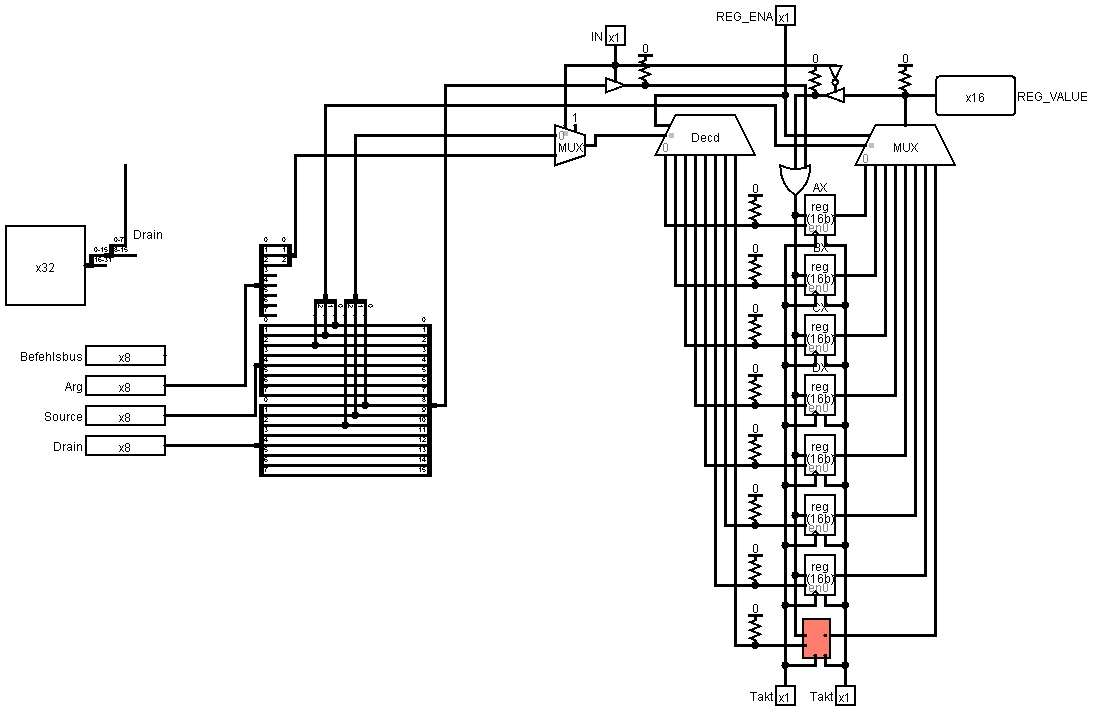
\includegraphics[scale=0.40]{circ}
\caption{Darstellung des RegisterwerkTODO}
\centering
\label{fig:register}
\end{figure}

\subsection{Register}
Register sind die schnellste Speichereinheit innerhalb einer CPU. Prozessoren besitzen eine vielfach höhere Ausführungsgeschwindigkeit als Arbeitsspeicher. Die CPU müsste ohne Register viele Taktzyklen auf Daten warten bevor sie diese verarbeiten könnte. Register bieten deshalb die Möglichkeit, sehr kleine Datenmengen mit einer sehr geringen Latenz prozessorintern lesen und schreiben zu können. Übliche Registergrößen sind 8,16,32 oder 64 Bit.\cite{mikroprozessortechnik2011} Sie werden aus Flip-Flops aufgebaut welche jeweils genau ein Bit speichern können, das heißt ein 64 Bit Register besteht aus 64 gemeinsam gesteuerten Flip-Flops.\cite{mikroprozessortechnik2011} Diese Art der Datenspeicherung hat allerdings auch einige Nachteile. So verbrauchen Register sehr viel Energie und Platz auf dem Prozessordie, es werden deshalb keine großen Speichermengen zur Verfügung gestellt. (Nachteile evtl streichen)

\subsubsection{Universalregister}
Es werden zwei Arten von Registergruppen unterschieden.In einem Universalregister kann ein Programm Werte und Variablen abspeichern.Sie stehen außerdem einem Programmierer von außen offen, das heißt er kann auf jedes Universalregister direkt zugreifen und seinen Wert verändern.

\subsubsection{Spezialregister}
Spezialregister werden von einer CPU für interne Zwecke genutzt. Oft sind in Prozessoren ähnliche Spezialregister zu finden. 

Der StackPointer(SP) ist ein Register welcher auf die aktuelle Position des Stacks im Speicher zeigt. Wenn der Befehl zu Speicherung eines Werts auf dem Stack ausgeführt wird inkrementiert die CPU automatisch, durch die interne Verschaltung des SP, den Wert des StackPointers. Dadurch zeigt das Register immer auf die nächste freie Speicheradresse im Stack.

Der InstructionPointer(IP) enthält die Adresse des nächsten Befehls im Programmspeicher der ausgeführt werden muss. Auch er wird nach der Abarbeitung eines Befehlszyklus als letzter Schritt inkrementiert. Dieses Register bietet allerdings die Möglichkeit einen anderen Wert zu laden. Das wird zur Realisierung von Sprüngen innerhalb des Programmcodes benötigt. 

Das Statusregister(SR) werden zur Ausführung von bedingten Sprunganweisungen gebraucht. Sie werden auch Flagregister genannt da die ALU, in Abhängigkeit der zuletzt ausgeführten Rechenoperation, einzelne Bit(Flags) setzen kann. Auf die einzelnen Flags und ihre Bedeutung wird im Abschnitt der ALU näher eingegangen
\subsection{Arithmetisch Logische Einheit}
\subsubsection{ALU-Konfigurationen}
%https://en.wikibooks.org/wiki/Microprocessor_Design/ALU#Example:_4-Bit_ALU
%https://en.wikibooks.org/wiki/Microprocessor_Design
\subsubsection{Arithmetische Operationen}
\subsubsection{Logische Operationen}
\subsection{Memory Management Unit(evtl)}
\subsection{Bussysteme}

\section{Speicher}
%https://de.wikipedia.org/wiki/Speicherhierarchie
\subsection{RAM/ROM}
\subsection{Stack}

\section{Befehlsausführung}
\subsection{Befehlszyklus}
\subsection{Schleifen}

\section{Besondere Ausführungsarten}
\subsection{Interrupts}
\subsection{Exceptions}
\subsection{Subroutinen}

\newpage

\section{Planung und Entwurf eines Prozessors}
Der Inhalt der bisherigen Arbeit handelte von den Komponenten einer CPU und deren Funktionsweißen. Um den dargestellten Inhalt praktischer Vermitteln zu können, wird nun mittels einer Simulationssoftware eine CPU von Grund auf erstellt. Dieser Prozessor stellt keinen Vergleich zu modernen Prozessoren her. Er soll lediglich die Funktionsweiße der essentiellsten Bauteile beschreiben und einfache Operationen wie Sprünge und Subroutinen unterstützen.
\subsection{Befehlsbreite}
Am Anfang der Planung jeder CPU steht die Festlegung der benötigten Befehlsbreite. Je nachdem welche Features eingebaut werden sollen kann der Befehlssatz eingeteilt werden. Logisim bietet die Möglichkeit, einen 32-Bit Bus zu nuzten. Zu Erklärungszwecken werden die 32-Bit wie folgt aufgeteilt:

\begin{table}[!htb]
\centering
\caption{Befehlsbus}
\label{Befehlsbus}
\begin{tabular}{|r|l|}
  \hline
  8-Bit & Opcode \\
  \hline
  8-Bit & Argument \\ 
  \hline
  16-Bit & Value\\
  \hline
  
\end{tabular}
\end{table}

\indent
\textbf{Opcode: } Der Opcode beinhaltet den Befehl welche die CPU als nächstes Ausführen soll(z.B. MOV oder ADD). Es werden nicht mehr als 8-Bit benötigt, da nicht viele Befehle vorhanden sein müssen um die Basisfunktionalität einer CPU zu erzielen.
\newline
\indent
\textbf{Argument: } Das Argument wird nicht bei jedem Befehl verwendet. Diese 8-Bit sind eine Hilfestellung für Operationen bei denen eine genauere Spezifikation der zu ausführenden Tätigkeit benötigt wird. Beispielsweise wird bei der arithmetischen Operation ADD mit Hilfe des Argumentes angegeben, in welches Register das Ergebnis gespeichert werden soll.
\newline
\indent
\textbf{Value: } Die verbleibenden 16-Bit werden als Wertangabe benutzt. Durch diese 16-Bit wird gleichzeitig die Befehlsbusbreite innerhalb des Prozessors festgelegt, das heißt der Prozessor kann mit Zahlen arbeiten welche innerhalb der 16-Bit Grenze liegen (ohne Vorzeichen maximal 65536). Einige Befehle in dieser CPU benötigen allerdings drei Parameter zur Ausführung. Um mit dem Argument drei Parameter bereitzustellen können die letzten 16-Bit in zwei 8-Bit Blöcke gespalten werden. Diese werden hier Quelle und Ziel genannt. Der Befehlssatz sieht bei diesen speziellen Befehlen folgendermaßen aus: 
\begin{table}[!htb]
\centering
\caption{Befehlsbus mit drei Parametern}
\label{Befehlsbus3P}
\begin{tabular}{|r|l|}
  \hline
  8-Bit & Opcode \\
  \hline
  8-Bit & Argument \\ 
  \hline
  8-Bit & Ziel\\
  \hline
  8-Bit & Quelle\\
  \hline
\end{tabular}
\end{table}
\newline
Befehle, welche diese Aufteilung benötigen sind zum Beispiel ALU-Operationen oder der MOV Befehl, welcher den Wert eines Register in ein anderes schiebt.

\subsection{Befehlssatz}

Der Befehlssatz beschreibt die Befehle, welche die CPU ausführen kann.
\newpage
\begin{table}[!htb]
\centering
\caption{Befehlssatz von VI-17}
\begin{tabular}{|r|l|}
  \hline
  00000000 & NOP \\
  \hline
  00000001 & MOV\\ 
  \hline
  00000010 & IN\\
  \hline
  00000011 & STO\\
  \hline
  00000100 & LEA\\
  \hline
  00000101 & PUSH \\ 
  \hline
  00000110 & POP\\
  \hline
  00000111 & -----\\
 \hline
  00001000 & ----- \\
  \hline
  00001001 & CALL\\ 
  \hline
  00001010 & RETURN\\
  \hline
  00001011 & ADD\\
  \hline 
 00001100 & SUB \\
  \hline
  00001101 & INC\\ 
  \hline
  00001110 & DEC\\
  \hline
  00001111 & COMP\\
  \hline
  00010000 & SHIFTL\\
  \hline
  00010001 & SHIFTR\\ 
  \hline
  00010010 & ROTL\\
  \hline
  00010011 & ROTR\\
  \hline
  00010100 & AND\\
  \hline
  00010101 & OR \\ 
  \hline
  00010110 & NOR\\
  \hline
  00010111 & NAND\\
  \hline
  00011000 & XOR\\
  \hline
  00011001 & XNOR \\
  \hline
  00011010 & JIT\\
  \hline
  00011011 & JIF\\
  \hline
  00011100 & JUMP\\
  \hline
\end{tabular}
\end{table}
\newpage
Die CPU soll die grundlegenden Aufgaben eines Prozessors erfüllen können. Die einzelnen Befehle des obigen Befehlssatzes werden nun kurz beschrieben.
\newline
\indent 
\textbf{00000000 NOP: }No Operation. Es wird keine Operation ausgeführt.
\newline
\indent 
\textbf{00000001 MOV: } Move. Überschreibt den Wert des Zielregisters mit dem Wert des Quellregisters. 


\subsection{Speicher}

\subsubsection{RAM/ROM}
\subsubsection{Stack}

\section{Implementierung einer Prozessorsimulation in Logisim}
\subsection{Logisim}
Logisim ist ein Open Source Werkzeug für den Entwurf und die Simulation digitaler Schaltungen. Es bietet die Möglichkeit, größere Schaltungen aus kleineren Schaltungen herzustellen. Damit ist es möglich, ganze Prozessoren in Logisim zu entwerfen. Ein solch einfacher Prozessor soll nun im Folgenden implementiert werden.
\subsection{Prozessor Komponenten}
Der Prozessor besteht aus fünf Hauptkomponenten:
\begin{itemize}
\item Control Unit - Steuerungseinheit
\item ALU - Arithmetisch Logische Einheit
\item Registersatz 
\item RAM/Stack
\item ROM
\end{itemize}

\textbf{Control Unit - Steuerungseinheit: } Die CU verarbeitet die Daten des Befehlsbusses und dekodiert die einzelnen Befehle, welche die CPU als nächstes ausführen muss. Der Befehlsbus wird mittels Komparatoren mit dem gesamtem Befehlssatz verglichen. Wenn ein Befehl gefunden wird sendet die CU die notwendigen Steuersignale an die einzelnen Komponenten des Prozessors, um zum Beispiel die Register zum beschreiben freizuschalten.

\begin{figure}[!htb]
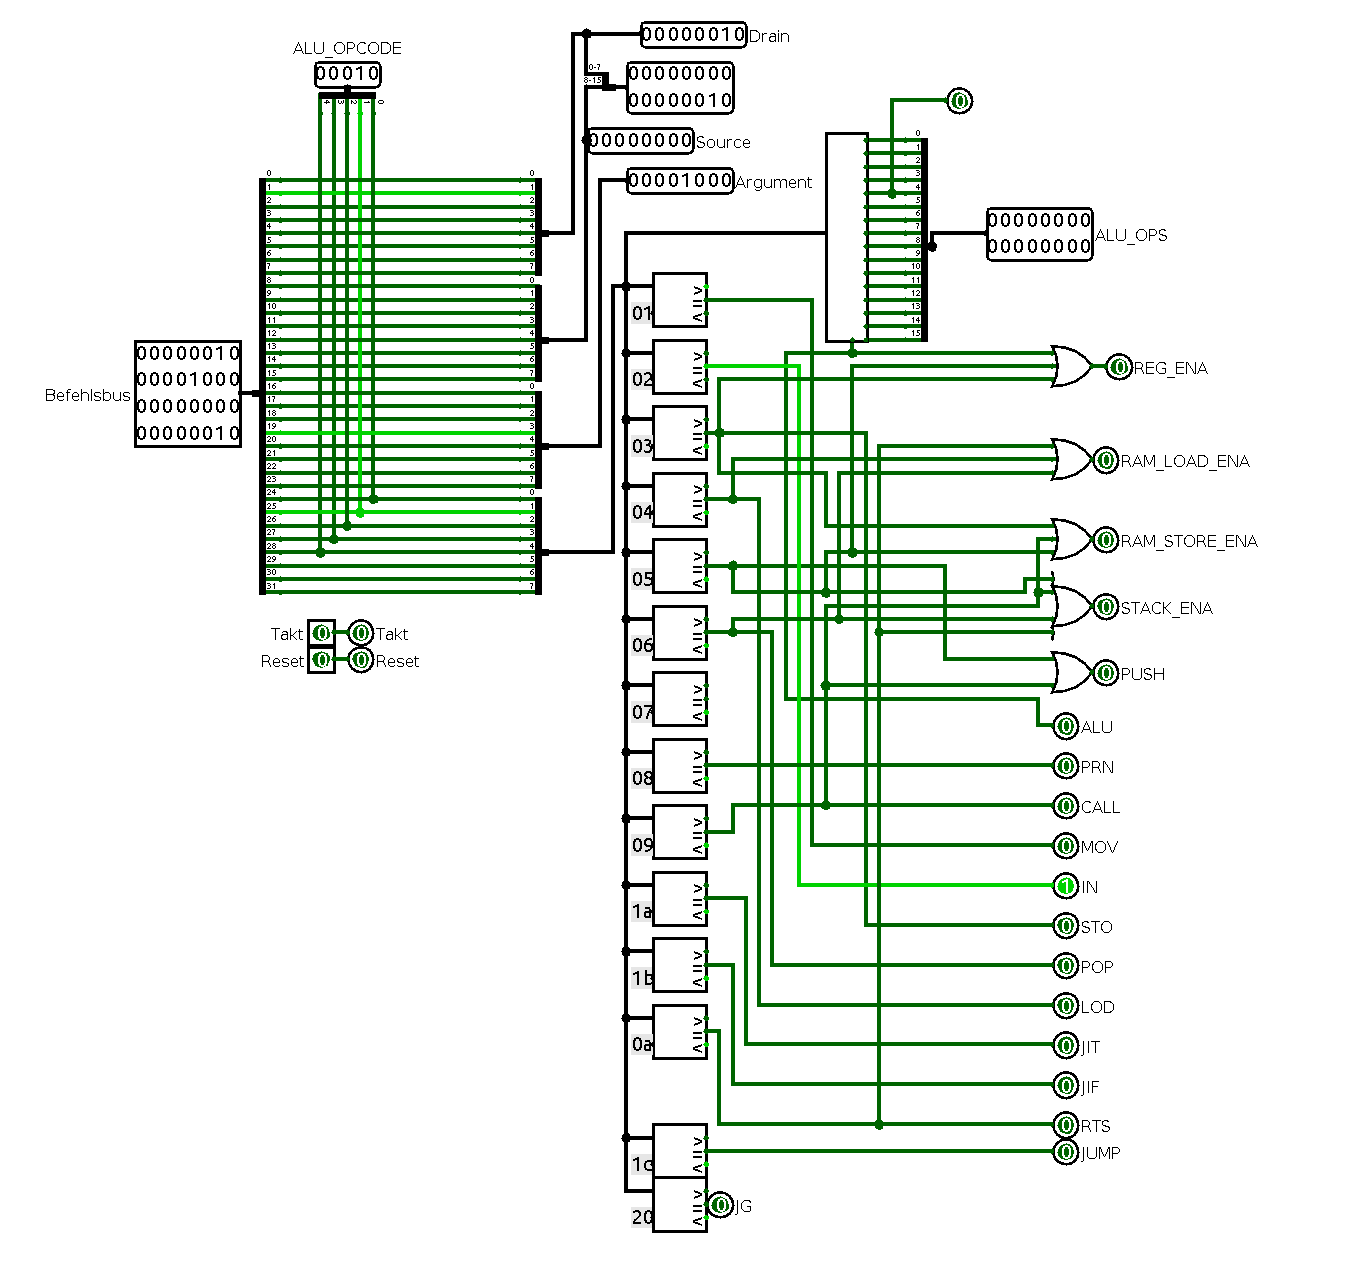
\includegraphics[scale=0.40]{cu}
\caption{Darstellung des Steuerwerks}
\centering
\label{fig:register}
\end{figure}

\newpage
\textbf{Registersatz: }
\begin{figure}[!htb]
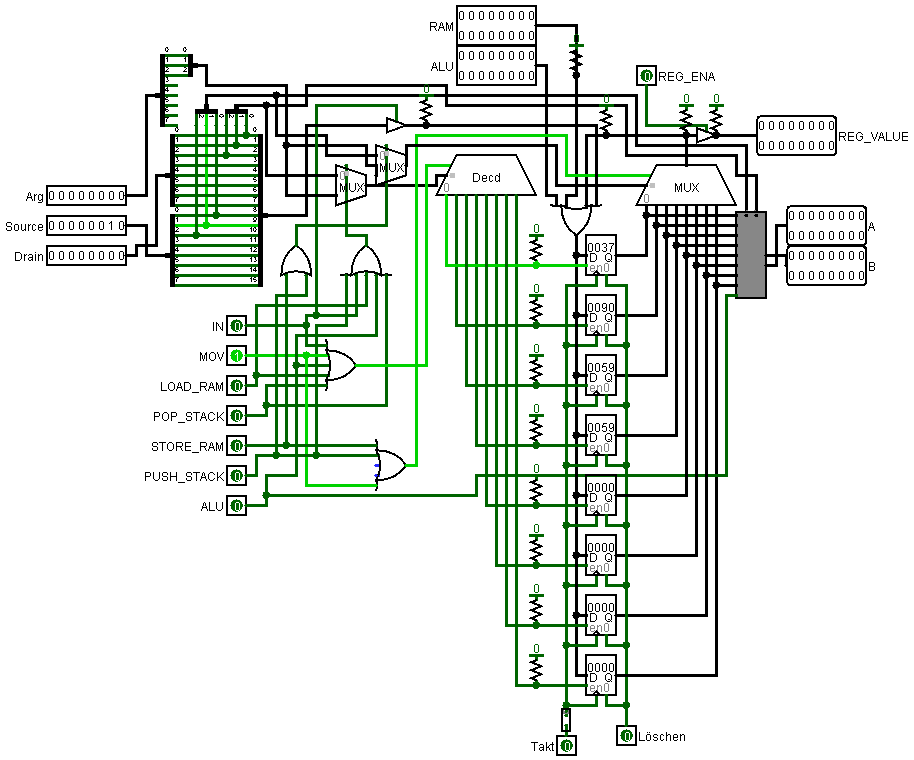
\includegraphics[scale=0.40]{register}
\caption{Darstellung des Registersatzes}
\centering
\label{fig:register}
\end{figure}

\subsection{Ausführung eines Assemblerprogrammes}

\newpage
\bibliography{Referenzen}

\end{document}



















